\subsection{Fourier-Analyse}
\begin{figure}
  \centering
  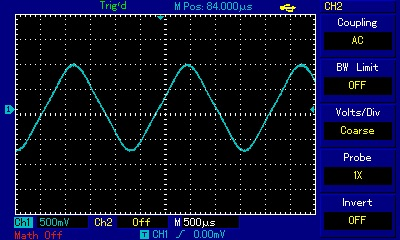
\includegraphics[width=0.7\textwidth]{bilder/dreieck.pdf}
  \caption{Ausgleichsgerade Dreieckspannung}
  \label{fig:fitdrei}
\end{figure}

\begin{figure}
  \centering
  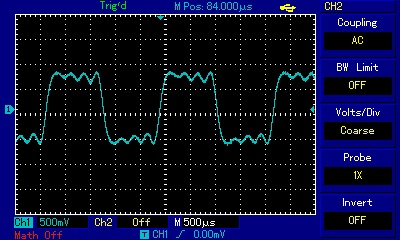
\includegraphics[width=0.7\textwidth]{bilder/rechteck.pdf}
  \caption{Ausgleichsgerade Rechteckspannung}
  \label{fig:fitrecht}
\end{figure}

\begin{figure}
  \centering
  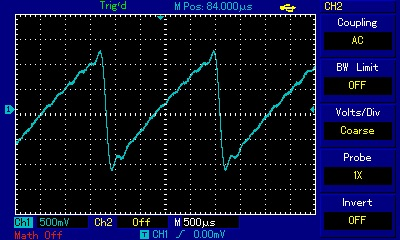
\includegraphics[width=0.7\textwidth]{bilder/saegezahn.pdf}
  \caption{Ausgleichsgerade Sägezahnspannung}
  \label{fig:fitsäge}
\end{figure}


\subsection{Fourier-Synthese}
In den Abbildungen \ref{fig:drei}, \ref{fig:recht} und \ref{fig:säge} sind die synthetisierten
Spannungskurven für die Dreick-, Rechteck- und Sägezahnspannung zu sehen.
Für die Dreieckspannung werden die Werte aus Tabelle \ref{tab:drei} verwendet.
\begin{table}
  \centering
  \begin{tabular}{c c c}
    \toprule
    $n$ & $U_\su{n}\,/\,\si{\milli\volt}$ & $U_\su{n, theo}\,/\,\si{\milli\volt}$ \\
    \midrule
    1 & 600   &    600  \\
    3 & 150   &    150  \\
    5 & 67    &    67   \\
    7 & 48    &    38   \\
    \bottomrule
  \end{tabular}
  \caption{Dreieckspannung der Oberwellen}
  \label{tab:drei}
\end{table}

\begin{figure}
  \centering
  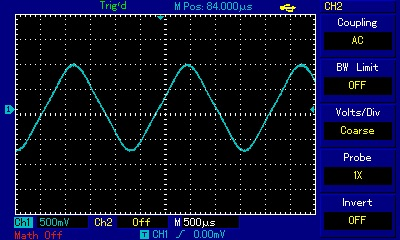
\includegraphics[width=0.6\textwidth]{bilder/dreieck.jpg}
  \caption{Dreieckspannung}
  \label{fig:drei}
\end{figure} \\

Für die Recht- und Sägezahnspannung werden die Werte aus Tabelle \ref{tab:rechtsäge}
benutzt.
\begin{table}
  \centering
  \begin{tabular}{c c c c}
    \toprule
    $n$ & $U_\su{n, Rechteck}\,/\,\si{\milli\volt}$ & $U_\su{n, Saegezahn}\,/\,\si{\milli\volt}$ &
     $U_\su{n, theo}\,/\,\si{\milli\volt}$ \\
    \midrule
    1 & 600   &  600  &  600  \\
    2 & -     &  300  &  300  \\
    3 & 200   &  200  &  200  \\
    4 & -     &  150  &  150  \\
    5 & 120   &  120  &  120  \\
    6 & -     &  100  &  100  \\
    7 &  86   &  86   &  86   \\
    8 & -     &  75   &  75   \\
    9 &  67   &  67   &  67   \\
   10 &  -    &  60   &  60   \\
    \bottomrule
  \end{tabular}
  \caption{Rechteck- / Sägezahnspannung der Oberwellen}
  \label{tab:rechtsäge}
\end{table}

\begin{figure}
  \centering
  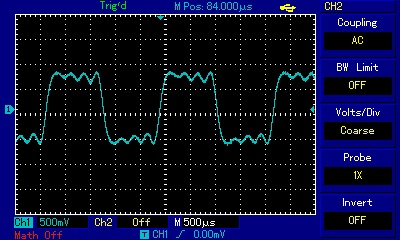
\includegraphics[width=0.6\textwidth]{bilder/rechteck.jpg}
  \caption{Rechteckspannung}
  \label{fig:recht}
\end{figure}

\begin{figure}
  \centering
  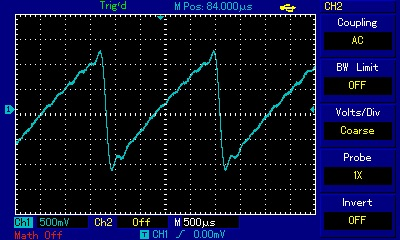
\includegraphics[width=0.6\textwidth]{bilder/saegezahn.jpg}
  \caption{Sägezahnspannung}
  \label{fig:säge}
\end{figure}
